\section{一次性口令:针对窃听的安全性}\label{sec:18-5}

如果对手能够窃听证明者和验证者之间的单独某一次交互,上一节中的口令协议就很容易被破坏。在这一节中,我们的目标是开发防窃听的身份识别协议。首先,我们需要定义存在窃听者的情况下的 ID 协议安全性。我们通过引入一个新的``窃听阶段"来加强攻击游戏 \ref{game:18-1}。在该阶段中,对手可以要求获取真正的证明者和真正的验证者之间的一些交互记录。更新后的攻击游戏如图 \ref{fig:18-7} 所示。

\begin{figure}
  \centering
  \tikzset{every picture/.style={line width=0.75pt}}

\begin{tikzpicture}[x=0.75pt,y=0.75pt,yscale=-0.9,xscale=0.9]

\draw  [fill={rgb, 255:red, 255; green, 255; blue, 255 }  ,fill opacity=1 ][line width=1.2] [general shadow={fill=black,shadow xshift=2.25pt,shadow yshift=-2.25pt}] (5,80) -- (115,80) -- (115,300) -- (5,300) -- cycle ;
\draw  [fill={rgb, 255:red, 255; green, 255; blue, 255 }  ,fill opacity=1 ][line width=1.2] [general shadow={fill=black,shadow xshift=2.25pt,shadow yshift=-2.25pt}] (340,80) -- (450,80) -- (450,300) -- (340,300) -- cycle ;

\draw   (25,250) -- (95,250) -- (95,290) -- (25,290) -- cycle ;

\draw  [->]  (60,290) -- (60,340) ;

\draw  [->]  (115,110) -- (338,110) ;
\draw  [->]  (115,150) -- (338,150) ;
\draw  [->]  (115,230) -- (338,230) ;
\draw  [<-]  (96,270) -- (340,270) ;

\draw (60,65) node   [align=left] {挑战者};
\draw (60,100) node    {$( vk,sk)\overset{\mathrm{R}}{\leftarrow } G()$};
\draw (60,270) node    {$V( vk)$};
\draw (225,175) node    {$\vdots $};
\draw (225,106.6) node [anchor=south] [inner sep=0.75pt]    {$vk$};
\draw (395,65) node   [align=left] {对手 $\mathcal{A}$};
\draw (65,337) node [anchor=west] [inner sep=0.75pt]   [align=left] {$\mathsf{accept}$ 或 $\mathsf{reject}$};

\draw (225,147) node [anchor=south] [inner sep=0.75pt]   [align=left] {$\text{对话}_1$};
\draw (225,227) node [anchor=south] [inner sep=0.75pt]   [align=left] {$\text{对话}_Q$};
\draw (225,267) node [anchor=south] [inner sep=0.75pt]   [align=left] {冒充尝试};


\end{tikzpicture}
  \caption{攻击游戏 \ref{game:18-2}}
  \label{fig:18-7}
\end{figure}

\begin{game}[安全的身份识别:窃听攻击]\label{game:18-2}
对于一个给定的身份识别协议 $\mathcal{I}=(G,P,V)$ 和一个给定的对手 $\mathcal{A}$,攻击游戏运行如下:
\begin{itemize}
	\item \emph{密钥生成阶段。}挑战者运行 $(vk,sk)\overset{\rm R}\leftarrow G()$,然后将 $vk$ 发送给对手 $\mathcal{A}$。
	\item \emph{窃听阶段。}对手请求若干条(比如 $Q$ 条)$P$ 与 $V$ 之间交互的记录。挑战者会运行 $Q$ 次 $P$ 与 $V$ 的交互,在其中的每一次中,$P$ 都以输入 $sk$ 初始化,$V$ 都以输入 $vk$ 初始化。挑战者将交互记录 $T_1,T_2,\dots,T_Q$ 发送给对手。
	\item \emph{冒充尝试。}如攻击游戏 \ref{game:18-1} 中一样,挑战者与 $\mathcal{A}$ 交互。挑战者遵循验证者的算法 $V$(以 $vk$ 为输入),而对手 $\mathcal{A}$ 会扮演证明者的角色,但不一定会遵循证明者的算法 $P$。
\end{itemize}
如果验证协议 $V$ 在交互结束时输出 $\mathsf{accept}$,我们就称对手 $\mathcal{A}$ 赢得了游戏。我们将 $\mathcal{A}$ 就
$\mathcal{I}$ 的优势定义为 $\mathrm{ID2}\mathsf{adv}[\mathcal{A},\mathcal{I}]$,即 $\mathcal{A}$ 赢得游戏的概率。
\end{game}

\begin{definition}\label{def:18-6}
如果对于所有的有效对手 $\mathcal{A}$,$\mathrm{ID2}\mathsf{adv}[\mathcal{A},\mathcal{I}]$ 的值都可忽略不计,我们就称识别协议 $\mathcal{I}$ \textbf{对窃听攻击是安全的(secure against eavesdropping attacks)}。
\end{definition}

\begin{snote}[保持 $vk$ 的机密性。]
攻击游戏 \ref{game:18-2} 中的对手得到了验证密钥 $vk$,这意味着 $vk$ 可以被视为公共信息。然而,我们提出的第一个窃听安全的 ID 协议要求验证者保持 $vk$ 的机密性。这就促成了一个攻击游戏 \ref{game:18-2} 的弱化版本,即挑战者不向对手发送 $vk$。当 $vk$ 被保密时,一个稍微有点复杂的情况是,我们现在必须允许对手进行多次冒充尝试。我们可以坚持要求这些冒充尝试按顺序进行,或者允许它们同时进行。在本章中,我们将假设它们是按顺序进行的。如果至少有一次冒充尝试被验证者接受,对手就赢得了游戏。

我们需要允许多次冒充尝试的原因是,现在,当 $vk$ 是机密的时候,与验证者的互动有可能泄露 $vk$ 的一些信息。这种更强的安全性定义能够排除一些显然不安全的协议,比如我们将会在练习 \ref{exer:18-10} 中讨论的那些。我们注意到,在攻击游戏 \ref{game:18-2} 中, $vk$ 是公开的,而多次尝试并不是必要的,因为对手可以模仿验证者本身。

除了这两点以外,攻击游戏 \ref{game:18-2} 的其余部分都没有变化。我们令 $\mathrm{wID2}\mathsf{adv}[\mathcal{A},\mathcal{I}]$ 为对手赢得这个较弱版本的攻击游戏的优势。在这种设置下安全的身份识别协议被称为是\textbf{弱安全的(weakly secure)}。
\end{snote}

\begin{definition}\label{def:18-7}
如果对于所有的有效对手 $\mathcal{A}$,$\mathrm{wID2}\mathsf{adv}[\mathcal{A},\mathcal{I}]$ 的值都可忽略不计,我们就称识别协议 $\mathcal{I}$ \textbf{对窃听攻击是弱安全的(weakly secure against eavesdropping attacks)}。
\end{definition}

\begin{snote}[有状态协议。]
上一节中的口令协议都是无状态的,即验证者和证明者在协议的不同调用之间不保持状态。然而,在本节中,我们提出的两个协议都是有状态的。

在一个有状态的协议中,每次调用协议后,数对 $(vk,sk)$ 都会发生变化:证明者 $P$ 会更新 $sk$,而验证者 $V$ 会更新 $vk$。然而,我们将假设 $V$ 只在输出 $\mathsf{accept}$ 时更新 $vk$。

我们现在考虑,如何修改攻击游戏 \ref{game:18-2} 以处理有状态协议。和之前一样,我们允许对手窃听 $P$ 和 $V$ 之间的多次对话。此外,我们还允许对手进行多次冒充尝试(不过,如果 $vk$ 不被保密,只考虑一次冒充尝试也就足够了)。但还有一个问题。在无状态的情况下,不失一般性,我们可以假设对手在进行任何冒充尝试之前获得了所有的交互记录。然而,在有状态协议中,情况不再是这样,我们必须允许对手交错进行窃听和冒充尝试。也就是说,现在,攻击游戏是分回合进行的。在每一轮中,对手可以选择以下两种行为中的一个:
\begin{itemize}
	\item \emph{窃听}:获得 $P$ 和 $V$ 之间的一次记录,然后,$P$ 更新 $sk$,$V$ 更新 $vk$,或者
	\item \emph{冒充}:进行冒充尝试,与 $V$ 进行交互。
\end{itemize}
此外,我们还假设,只要有一次冒充尝试成功,攻击游戏就会结束(在这种情况下,对手赢得游戏)。回顾一下,我们假设 $V$ 在冒充尝试失败时不会更新 $vk$,这就保证了,在窃听回合中,$P$ 和 $V$ 会保持恰当的同步。
\end{snote}

\subsection{基于 PRF 的一次性口令:HOTP 和 TOTP}\label{subsec:18-5-1}

最简单的防窃听攻击的 ID 协议被称为\textbf{一次性口令(one-time password)} 协议。这些协议类似于 \ref{sec:18-3} 节中的基本口令协议,只是在每次调用协议后,口令都会发生变化。

我们首先描述一个弱安全的协议,称为\textbf{基于哈希的一次性口令 (hash-based one-time password, HOTP)}。令 $F$ 是一个定义在 $(\mathcal{K},\mathbb{Z}_N,\mathcal{Y})$ 上的 PRF,其中 $N$ 是某个大整数,比如 $N=2^{128}$。这个 $F$ 被用于在每次成功交互后更新口令。HOTP 协议 $\mathtt{HTOP}=(G,P,V)$ 运行如下:
\begin{itemize}
	\item $G$:随机选取一个 $k\overset{\rm R}\leftarrow\mathcal{K}$ 并输出 $sk:=(k,0)$ 和 $vk:=(k,0)$,
	\item 算法 $P$ 被赋予 $sk$,算法 $V$ 被赋予 $vk$,并按如下方式交互:
	\begin{enumerate}
		\item $P\big(sk=(k,i)\big)$:向 $V$ 发送 $r:=F(k,i)$,并且设置 $sk\leftarrow (k,i+1)$,
		\item $V\big(vk=(k,i)\big)$:如果来自 $P$ 的 $r$ 满足 $r=F(k,i)$,输出 $\mathsf{accept}$ 并设置 $vk\leftarrow(k,i+1)$。否则输出 $\mathsf{reject}$。
	\end{enumerate}
\end{itemize}
这里 $vk$ 和 $sk$ 都必须保密,因此 HOTP 对窃听的安全性很低。请注意,整数 $N$ 被选用一个极大的数,以至于在实践中,计数器 $i$ 永远不会被重复使用。HOTP 的实现通常使用 HMAC-SHA256 作为底层的 PRF,其输出被截断到所需的大小,通常是六位小数,如图 \ref{fig:18-8} 所示。

\begin{figure}
  \centering
  \subfigure[RSA SecureID 令牌]{
  	  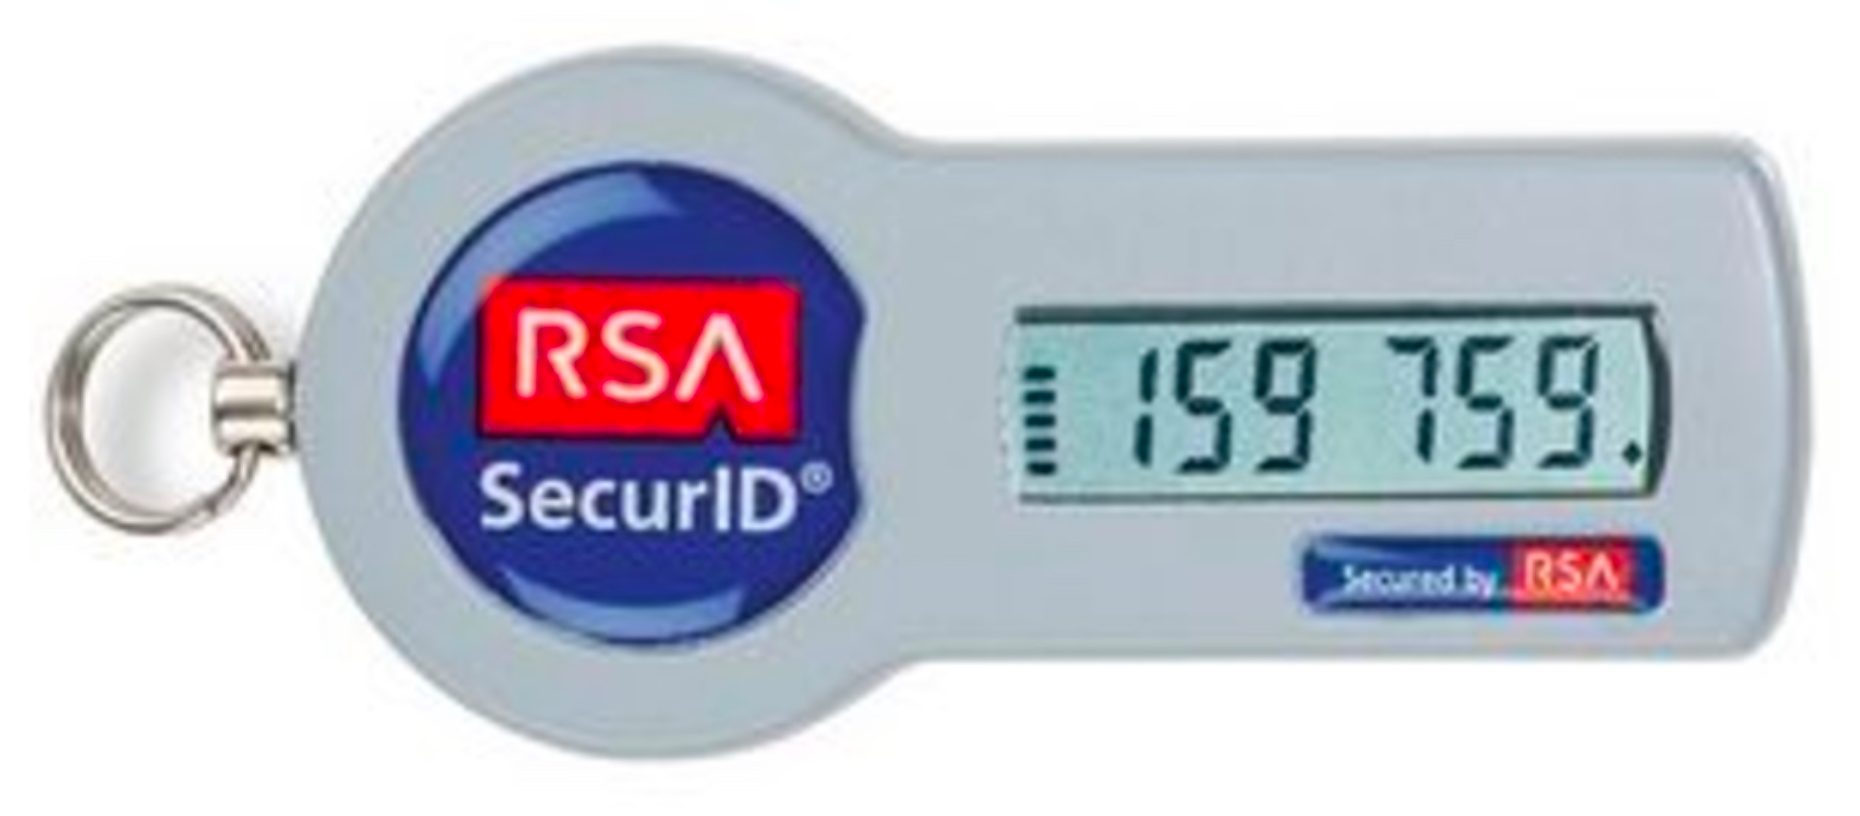
\includegraphics[width=0.3\linewidth]{figures/chapter18/fig8-a.png}
  	  \label{fig:18-8-a}
  }
  \qquad\qquad\qquad\qquad
  \subfigure[Google 认证器]{
      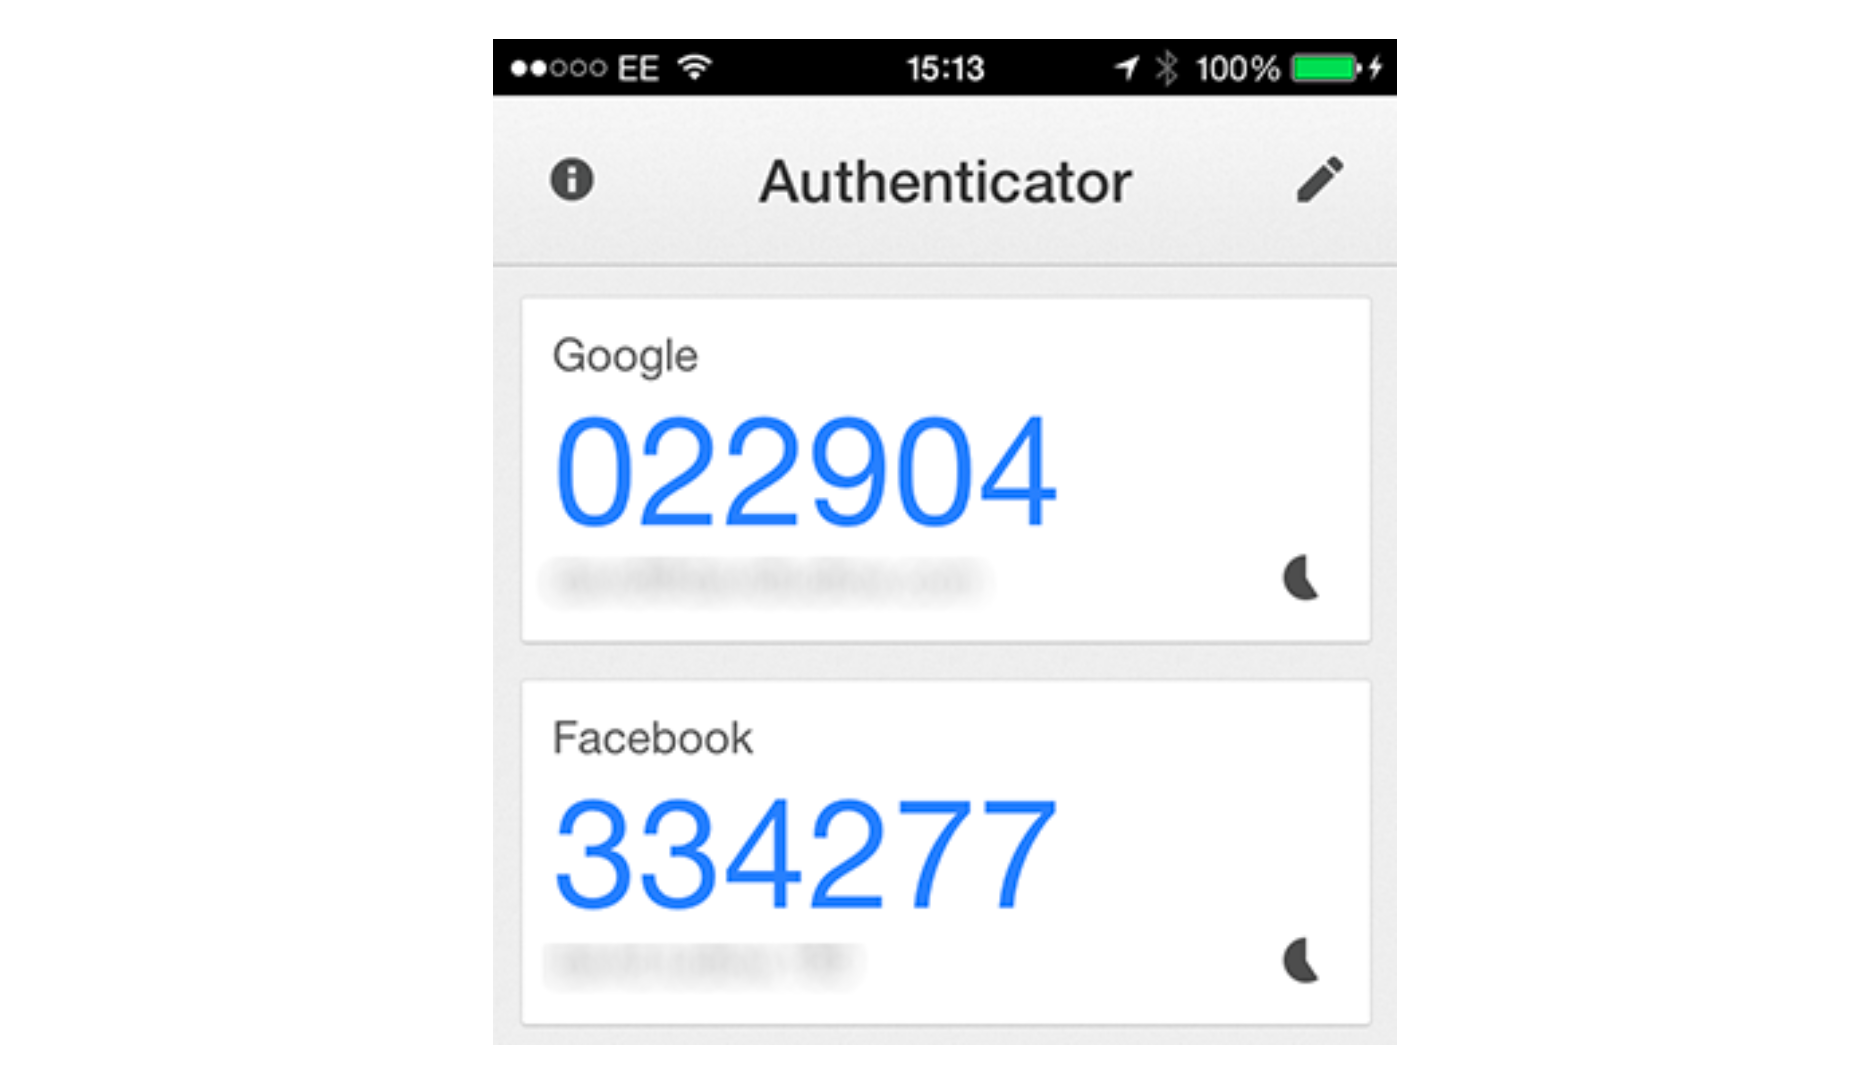
\includegraphics[width=0.3\linewidth]{figures/chapter18/fig8-b.png}
      \label{fig:18-8-b}
  }
  \caption{TOTP实现}
  \label{fig:18-8}
\end{figure}

\begin{theorem}\label{theo:18-4}
令 $F$ 是一个定义在 $(\mathcal{K},\mathbb{Z}_N,\mathcal{Y})$ 上的安全的 PNF,其中 $N$ 和 $|\mathcal{Y}|$ 都是超多项式的。那么,ID 协议 \texttt{HOTP} 对窃听是弱安全的。
\end{theorem}

\begin{proof}[证明简述]
由于 $F$ 是一个安全的 PRF,那么在攻击游戏 \ref{game:18-2} 中,对手无法区分使用 PRF 的挑战者和使用随机函数 $f:\mathbb{Z}_N\to\mathcal{Y}$ 的挑战者。此外,当挑战者使用随机函数 $f$ 时,冒充尝试的成功概率最大是 ${1}/{|\mathcal{Y}|}$。而由于 $|\mathcal{Y}|$ 是超多项式的,所以该值可忽略不计。此外,由于 $N$ 很大,在任何可行的攻击中,计数器的值都不会``环绕一圈"。
\end{proof}

HOTP 可以被用在汽车钥匙扣系统中,用于以无线方式解锁汽车,就像本章导言部分讨论的那样。秘密的 PRF 密钥 $k$ 会被存储在钥匙扣和汽车上。每当用户按下钥匙扣上的一个按钮时,钥匙扣就将内部计数器 $i$ 的值递增 $1$,并将得到的一次性口令连同计数器 $i$ 一起发送给汽车。需要注意的是,汽车必须确保收到的计数器值大于汽车当前的计数器值。

HOTP 也可以被远程网络服务器用于验证人类用户的身份。用户会得到一个安全令牌,它看起来就像图 \ref{fig:18-8-a} 中所展示的那样,显示一个 $6$ 位数的一次性口令。用户需要在她的网络浏览器中输入这个口令,以此向远程服务器证明身份。然后,这个一次性口令就会被发送到远程服务器上进行验证。下一次,当用户想再次向服务器提交验证时,她首先按下令牌上的一个按钮,使计数器 $i$ 增加 $1$。这就把令牌推进到下一个一次性口令,并更新屏幕上显示的 $6$ 位数的数值。

由于若干原因,HOTP 系统会带来很多问题。首先,在远程网络服务器的场景中,我们希望尽可能的减少用户需要输入的字符数。特别是,我们不希望要求用户在输入 $6$ 位口令的同时还要输入当前的计数器值。然而,在令牌和远程服务器不同步的情况下,计数器的值是必然需要同步的。如果我们能使用一个双方都知道的隐式计数器,情况将会变得更加友好。如下文所述,当前时间恰好就可以作为一个隐式的计数器。

其次,HOTP 还有一个安全性问题。在 HOTP 中,一次性口令只有在用户启动协议时才会被更新。如果用户不经常认证,比如一个月才使用一次,那么每个一次性口令都会在整个月内有效。攻击者如果以某种方式获得了用户当前的一次性口令,就可以把它卖给任何想冒充用户的人。那么,只要用户还没有对服务器发出新的认证请求,买家就可以在任何时候使用购买的口令,因为它一直是有效的。

\subsubsection{基于时间的一次性口令}\label{subsubsec:18-5-1-1}

一个更好的一次性口令方案被称为\textbf{基于时间的一次性口令 (time-based one-time password, TOTP)}。在 TOTP 中,无论用户是否认证,计数器 $i$ 都会每 $30$ 秒自增一次。这意味着,每个一次性口令都只在短时间内有效。当使用图 \ref{fig:18-8-b} 这样的硬件令牌时,显示屏每 $30$ 秒就会改变一次,并向用户展示最新的一次性口令。因此现在,令牌上并没有按钮。

每当用户向远程服务器发起认证请求时,服务器就会用当前时间来确定计数器 $i$ 的值,然后验证用户提供的 $r:=F(k,i)$ 是否正确。考虑到服务器和令牌之间的可能存在时钟偏移,服务器会接受 $\{F(k,(i-c)),\dots,F(k,(i+c))\}$ 中的任何一个口令作为有效的口令,其中 $c$ 是某个小的正整数,比如 $c=5$。在 $2c+1$ 的时钟偏移窗口内,服务器会拒绝以前使用过的口令,以此来防止重放攻击。

图 \ref{fig:18-8-a} 是 TOTP 的一个硬件令牌实现。在令牌设置时,一个秘密 PRF 密钥会被加载到令牌中,用于生成一个 $6$ 位数的一次性口令。服务器也持有相同的 PRF 密钥。硬件令牌内部有一个电池,可以为设备提供长达数年的供电。当电池耗尽时,令牌就会失效。

图 \ref{fig:18-8-b} 是一个智能手机上的 TOTP 应用程序。用户通过输入或扫描二维码将秘密 PRF 密钥加载到应用程序中。该应用可以管理用户在多个系统中的一次性口令,如图所示,该应用正在管理 Google 和 Facebook 的一次性口令。

\subsection{S/key 系统}\label{subsec:18-5-2}

TOTP 要求服务器始终保持其存储的验证密钥 $vk$ 的机密性。如果对手窃取了 $vk$ 而没有被发现,所有的安全性都会丧失。这实际上已经发生在了一些广为人知的案例中。

一个被称为 S/key 的系统取消了这种限制。然而,在 S/key 系统中,每对 $(vk,sk)$ 都只能被使用有限次,然后就必须重新生成一对新的。令 $n$ 是一个预设的多项式边界整数,比如 $n=10^6$,它表示一个数对 $(vk,sk)$ 能被使用的最大次数。

在 \ref{sec:14-3} 节中,我们曾经介绍过哈希链的概念,我们这里就要使用它。回顾一下,令 $H:\mathcal{X}\to\mathcal{X}$ 是一个函数。对于 $j\in\mathbb{Z}_{>0}$,我们用 $H^{(j)}(x)$ 表示 \textbf{$H$ 的第 $j$ 次迭代($j$-th iterate of $H$)},即 $H^{(j)}(x):=H(H(H(\cdots(x)\cdots)))$,其中 $H$ 被重复计算了 $j$ 次。我们令 $H^{(0)}(x):=x$。

\begin{snote}[S/key 协议。]
可被调用 $n$ 次的协议 $\mathtt{Skey}_n=(G,P,V)$ 运行如下:
\begin{itemize}
	\item $G$:随机选取一个 $k\overset{\rm R}\leftarrow\mathcal{X}$,输出 $sk:=(k,n)$,$vk:=H^{(n+1)}(k)$,
	\item 算法 $P$ 被赋予 $sk$,算法 $V$ 被赋予 $vk$,并按如下方式交互:
	\begin{enumerate}
		\item $P\big(sk=(k,i)\big)$:将 $t:=H^{(i)}(k)$ 发送给 $V$,并且设置 $sk\leftarrow(k,i-1)$,
		\item $V(vk)$:如果来自 $P$ 的 $t$ 满足 $vk=H(t)$,则输出 $\mathsf{accept}$,并设置 $vk\leftarrow t$。否则输出 $\mathsf{reject}$。
	\end{enumerate}
\end{itemize}
该协议如图 \ref{fig:18-9} 所示。在第一次调用时,证明者者向验证者发送口令 $H^{(n)}(k)$。在第二次调用中,证明者会发送 $H^{(n-1)}(k)$,以此类推。每个口令都只能使用一次。显然,经过 $n$ 次调用后,证明者的一次性口令就用完了,这时,证明者就不能再向验证者认证了,必须生成一个新的 $(vk,sk)$ 对。
\end{snote}

\begin{figure}
  \centering
  \tikzset{every picture/.style={line width=0.75pt}}

\begin{tikzpicture}[x=0.75pt,y=0.75pt,yscale=-1,xscale=1]

\draw  [->]  (20,30) -- (67,30) ;
\draw  [->]  (75,30) -- (197,30) ;
\draw  [->]  (205,30) -- (297,30) ;
\draw  [->]  (305,30) -- (397,30) ;
\draw  [->]  (405,30) -- (497,30) ;

\draw  [->]  (205,85) -- (205,38) ;
\draw  [->]  (305,85) -- (305,38) ;
\draw  [->]  (405,85) -- (405,38) ;
\draw  [->]  (505,85) -- (505,38) ;

\draw  [fill={rgb, 255:red, 0; green, 0; blue, 0 }  ,fill opacity=1 ] (71,30) .. controls (71,27.79) and (72.79,26) .. (75,26) .. controls (77.21,26) and (79,27.79) .. (79,30) .. controls (79,32.21) and (77.21,34) .. (75,34) .. controls (72.79,34) and (71,32.21) .. (71,30) -- cycle ;
\draw  [fill={rgb, 255:red, 0; green, 0; blue, 0 }  ,fill opacity=1 ] (201,30) .. controls (201,27.79) and (202.79,26) .. (205,26) .. controls (207.21,26) and (209,27.79) .. (209,30) .. controls (209,32.21) and (207.21,34) .. (205,34) .. controls (202.79,34) and (201,32.21) .. (201,30) -- cycle ;
\draw  [fill={rgb, 255:red, 0; green, 0; blue, 0 }  ,fill opacity=1 ] (301,30) .. controls (301,27.79) and (302.79,26) .. (305,26) .. controls (307.21,26) and (309,27.79) .. (309,30) .. controls (309,32.21) and (307.21,34) .. (305,34) .. controls (302.79,34) and (301,32.21) .. (301,30) -- cycle ;
\draw  [fill={rgb, 255:red, 0; green, 0; blue, 0 }  ,fill opacity=1 ] (401,30) .. controls (401,27.79) and (402.79,26) .. (405,26) .. controls (407.21,26) and (409,27.79) .. (409,30) .. controls (409,32.21) and (407.21,34) .. (405,34) .. controls (402.79,34) and (401,32.21) .. (401,30) -- cycle ;
\draw  [fill={rgb, 255:red, 0; green, 0; blue, 0 }  ,fill opacity=1 ] (16,30) .. controls (16,27.79) and (17.79,26) .. (20,26) .. controls (22.21,26) and (24,27.79) .. (24,30) .. controls (24,32.21) and (22.21,34) .. (20,34) .. controls (17.79,34) and (16,32.21) .. (16,30) -- cycle ;
\draw  [fill={rgb, 255:red, 0; green, 0; blue, 0 }  ,fill opacity=1 ] (501,30) .. controls (501,27.79) and (502.79,26) .. (505,26) .. controls (507.21,26) and (509,27.79) .. (509,30) .. controls (509,32.21) and (507.21,34) .. (505,34) .. controls (502.79,34) and (501,32.21) .. (501,30) -- cycle ;

\draw  [draw opacity=0][fill={rgb, 255:red, 255; green, 255; blue, 255 }  ,fill opacity=1 ] (117.5,25) -- (157.5,25) -- (157.5,35) -- (117.5,35) -- cycle ;
\draw  [dash pattern={on 0.84pt off 2.51pt}]  (117.5,30) -- (157.5,30) ;

\draw (20,22.6) node [anchor=south] [inner sep=0.75pt]    {$k$};
\draw (75,22.6) node [anchor=south] [inner sep=0.75pt]    {$H( k)$};
\draw (205,22.6) node [anchor=south] [inner sep=0.75pt]    {$H^{( n-2)}( k)$};
\draw (305,22.6) node [anchor=south] [inner sep=0.75pt]    {$H^{( n-1)}( k)$};
\draw (405,22.6) node [anchor=south] [inner sep=0.75pt]    {$H^{( n)}( k)$};
\draw (505,22.6) node [anchor=south] [inner sep=0.75pt]    {$H^{( n+1)}( k)$};
\draw (205,88) node [anchor=north] [inner sep=0.75pt]   [align=left] {口令 \#3};
\draw (305,88) node [anchor=north] [inner sep=0.75pt]   [align=left] {口令 \#2};
\draw (405,88) node [anchor=north] [inner sep=0.75pt]   [align=left] {口令 \#1};
\draw (505,88.4) node [anchor=north] [inner sep=0.75pt]    {$vk$};


\end{tikzpicture}
  \caption{S/key 协议}
  \label{fig:18-9}
\end{figure}

\begin{snote}[S/key 的安全性。]
我们声称,即使 $vk$ 被公开了,S/key 仍然是安全的。因此,S/key 对窃听是完全安全的,相比之下,\texttt{HOTP} 只是弱安全的。

对 S/key 的分析要求 $H:\mathcal{X}\to\mathcal{X}$ 在 $n$ 次迭代中都是 \ref{def:14-5} 意义上的单向函数。回顾一下,这意味着,对于所有的 $j=1,\dots,n$,给定 $y\leftarrow H^{(j)}(k)$ 作为输入,其中 $k\overset{\rm R}\leftarrow\mathcal{X}$,都很难找到一个 $H^{-1}(y)$ 中的元素。回顾一下,我们在练习 \ref{exer:14-15} 中表明,一个单向函数 $H$ 在 $n$ 次迭代中不一定是单向的,就算 $n=2$ 也是如此。然而,标准的密码学哈希函数,如 SHA256,在合理的 $n$ 值上确实是单向的,比如 $n\leq 10^{6}$ 时。
\end{snote}

\begin{theorem}\label{theo:18-5}
令 $H:\mathcal{X}\to\mathcal{X}$ 是一个 $n$ 次迭代上的单向函数。则身份识别协议 $\mathtt{Skey}_n$ 对窃听是安全的。
\end{theorem}

\begin{proof}[证明简述]
既然 $vk$ 是公开的,我们就可以假设对手窃听了多次(比如说 $Q$ 次)对话,然后进行了一次冒充尝试。我们事先不知道 $Q$ 是多少,但我们可以猜测它的值。我们从迭代的单向挑战者那里请求 $y\leftarrow H^{(n-Q+1)}(k)$,并使用 $y$ 来生成与初始验证密钥 $vk=H^{(n+1)}(k)$ 有关的 $Q$ 个有效对话。如果我们对 $Q$ 的猜测是正确的,并且对手成功地进行了冒充尝试,对手将为我们找到 $y$ 的原像。因此,如果对手能以概率 $\epsilon$ 成功冒充,我们就能以 $\epsilon/n$ 的概率赢得攻击游戏 \ref{game:14-1}。
\end{proof}

\begin{remark}\label{remark:18-1}
为了防御如 \ref{sec:18-7} 节所讨论的那类针对 $H$ 的预处理攻击,算法 $G$ 可以在设置时选择一个公共盐,并在每次评估 $H$ 时都将这个盐作为前缀添加到输入中。此外,为了避免 \ref{exer:14-17} 中所示的攻击,我们建议在哈希链的每一步中都使用不同的哈希函数。\cite{kogan2017t} 分析了这种防御。
\end{remark}

\begin{snote}[S/key 的麻烦。]
在每次认证尝试中,验证者 $P$ 都必须向 $V$ 发送一个元素 $t\in\mathcal{X}$。为了使 $H$ 是单向的,集合 $\mathcal{X}$ 必须很大,因此 $t$ 不能像 TOTP 系统中那样是一个 $6$ 位数。在实践中,$t$ 至少需要有 $128$ 位,以确保 $H$ 是单向的。这使得,当使用 S/key 作为一次性口令方案时,用户需要手动输入口令,这是很不方便的。将一个 $128$ 位的 $t$ 编码为可打印的字符,至少需要 $22$ 个字符。
\end{snote}